\chapter{Programación}


\section{Introducción}

\subsection{¿Cómo resolver un problema de Ingeniería por computadora?}

El ingeniero, se caracteriza por resolver problemas de la vida cotidiana mediante el ingenio humano. En éste caso, se recompilaron algunos métodos para atender a éstas necesidades, con las siguientes herramientas de programación:

\subsubsection{MatLab}

MATLAB combina un entorno de escritorio perfeccionado para el análisis iterativo y los procesos de diseño con un lenguaje de programación que expresa las matemáticas de matrices y arrays directamente \autocite{holly2007matlab}.

\subsubsection{Ejemplo de MATLAB}

Una demostración del algoritmo de Lanczos en la matriz (-1, 2, -1)

    \FrameTBStyle{matlab}
    \begin{lstlisting}[style=matlabFrameTB, gobble=4]
n = 4; 
A = gen_der2_mat(n); 

[Q,T]=lanczos(A);

disp('Q^T Q es igual a' ); 
(Q.') * Q 
disp( 'A*Q debe ser igual a Q T, la norma de la diferencia entre las dos matrices es' ); 
norm( A * Q - Q * T )
    \end{lstlisting}

\subsection{AutoCad}

\begin{definition}[Diseño]
  Es la delineación de una idea, las descripción de la forma de un sistema y preparación de los bosquejos preliminares y/o planos para un sistema que se va a producir.
\end{definition}

\begin{definition}[Diseño en la ingeniería]
  Es un proceso de toma de decisiones, diseñar es concebir, innovar, crear, uno puede generar totalmente un nuevo sistema o modificar y reamoldar objetos existentes en forma nueva, para mejorar su aprovechamiento o su funcionamiento.
\end{definition}

\subsubsection{Etapas del diseño}
Podemos identificar ciertos pasos para empezar a diseñar:
\begin{enumerate}
  \item Identificación de la necesidad
  \item Definición de la tarea (meta)
  \item Especificación de la tarea
  \item Idealización
  \item Conceptualización
  \item Análisis
  \item Prueba experimental
  \item Descripción del diseño
  \item Diseño para producción
\end{enumerate}

\subsubsection{Relación entre el dibujo y diseño}

El diseño de ingeniería utiliza el dibujo como el medio para comunicar y documentar ideas \autocite{li2012gamicad}.

Los dibujos de ingeniería presentan información para decenas, incluso cientos de personas, como son ingenieros, gerentes, mecánicos, instaladoes, etc.

El \textbf{Dibujo asistido por computadora} es un lenguaje de las computadora es numérico, sin embargo resulta más fácil comprender dichos valores cuando van acompañados de dibujo gráfico o imágen.

Los dibujos de ingeniería elaborados con el auxilio de la computadora son un medio importante para comprobar la valide< de los números de la base de datos, ya que es más fácil verificar una imágen que cincuenta hojas de números.

El termino \textbf{CAD} proviene de las siglas inglesas \texttt{Computer Aided Design} cuya traducción es diseño asistido por computadora, esta tecnología surge sobre los años de 1946 en el MIT.
El CAD es una técnica de análisis, una forma de modelar las cualidades de un producto antes de que en verdad se construya.

En general, cualquier sistema CAD debe involucrar dos aspectos muy importantes, un conjunto de datos numéricos (base de datos) y un modelo gráfico.

Las ventajas son evitar tareas tediosas, disminución del tiempo, disminución de los errores, eliminación de prototipos y alta rentabilidad.

\subsection{C}

Hecho principalmente para la fluidez de programación en sistemas Unix. Se usa también para el desarrollo de otros sistemas operativos como Windows o GNU/Linux. Igualmente para aplicaciones de escritorio como GIMP, cuyo principal lenguaje de programación es C \autocite{andersen1994program}.

De la misma forma, es muy usado en aplicaciones científicas (para experimentos informáticos, físicos, químicos, matemáticos, entre otros, parte de ellos conocidos como modelos y simuladores), industriales (industria robótica, cibernética, sistemas de información y base de datos para la industria petrolera y petroquímica. Predominan también todo lo que se refiere a simulación de máquinas de manufactura), simulaciones de vuelo (es la más delicada, ya que se tienen que usar demasiados recursos tanto de hardware como de software para desarrollar aplicaciones que permitan simular el vuelo real de una aeronave). Se aplica por tanto, en diversas áreas desconocidas por gran parte de los usuarios noveles.

\subsubsection{Ejemplo en C}

    \FrameTBStyle{c}
    \begin{lstlisting}[style=cFrameTB, gobble=4]
#include <conio.h>
#include <ctype.h>
#include <stdio.h>

int main() {
    char numero;
    fputs("Introduzca un numero entero par: ", stdout);

    scanf("%c", &numero);
    if (!isdigit(numero)) {
        fputs("Error: numero no valido.\n", stderr);
        return -1;
    }

    for (int i = 1; numero % 2 == 0; ++i) {
        printf("%.3d| %d/2 =", i, numero);
        numero /= 2;
        printf("%d\n", numero);
    }

    printf("No se puede seguir dividiendo: El numero %d es impar.\n", numero);
    getch();

    return 0;
}
    \end{lstlisting}

    \section{¿Qué es un algoritmo?}

Cuando los algoritmos se definen rigurosamente en la literatura informática (que sólo ocurre raramente), generalmente se identifican con máquinas abstractas, modelos matemáticos de computadoras, a veces idealizados al permitir el acceso a la ``memoria ilimitada''.) Esto no cuadra con las intuiciones sobre los algoritmos, la forma en que son interpretados y aplicados en los resultados sobre ellos \autocite{moschovakis2001algorithm}; 

La cuestión es saber cuándo, los algoritmos son definiciones recursivas mientras que hay otras que son implementaciones de modelos de máquinas, el cual involucra un tipo especial de algoritmos \autocite{gurevich2012algorithm}. Aún así podemos basarnos de una definición que describa una introducción a los algoritmos:

    \begin{definition}[Algoritmo]
        Es un bloque de construcción de la informática que se define desde un punto de vista intuitivo y pragmático, a través de una lente metodológica de la filosofía en lugar de la computación formal. El tratamiento extrae propiedades de abstracción, control, estructura, finitud, mecanismo efectivo e imperatividad, y aspectos intencionales de la meta y las condiciones previas. 
    \end{definition}

El enfoque en el algoritmo como un objeto conceptual robusto obvia cuestiones de corrección y minimidad \autocite{hill2016algorithm}. Ni la articulación de un algoritmo ni el proceso dinámico constituyen el algoritmo en sí. 

El análisis de las implicaciones en la ciencia de la computación y la filosofía revela resultados inesperados, nuevas preguntas y nuevas perspectivas sobre las preguntas actuales, incluida la relación entre nuestros algoritmos construidos informalmente y las máquinas de Turing. La exploración en términos del pensamiento filosófico y computacional actual invita a nuevos desarrollos.

Un algoritmo debe tener ciertas cualidades para que pueda ser programado:

\begin{enumerate}
    \item Debe tener cero o más datos de entrada
    \item Debe contemplar uno o más datos de salida
    \item Cada paso debe estar definido con exactitud
    \item Ha de ser finito, el algoritmo debe finalizar tras la ejecución de un número finito de pasos
    \item Debe ser efectivo, es decir cada uno de sus pasos debe ejecutarse en un determinado tiempo (ojalá el menor) con recursos limitados
\end{enumerate}

\subsubsection{Ejemplo}


    \FrameTBStyle{python}
    \begin{lstlisting}[style=pythonFrameTB, gobble=4]
    import numpy as np # Unnecessary import

    a, b = 69., .420

    def f(a: float, b: float) -> float:
        r"""
        Sum two numbers

        Parameters
        ----------
        a: first number
        b: second number

        Returns
        -------
        the sum of 'a' and 'b'
        """

        return a + b

    c = f(a, b)

    print('{:f} + {:f} equals {:f}'.format(a, b, c))
    \end{lstlisting}

En éste pedazo de código con el lenguaje de programación de \textit{Python}, es una interacción directa con la terminal, mas no con la salida. Se definen las variables \texttt{a} y \texttt{b} que son \texttt{float} para que al ingresar la entrada de aquellos valores, me resulte la adición, de manera que obtenermos un nuevo valor \texttt{c}.

Nosotros buscamos que al ingresar los dos valores, en la terminal me aparezca un mensaje diciendo:

\begin{equation}
    a+b=c
\end{equation}

Cumple con la definición de algoritmo, ya que hicimos una secuencia de instrucciones para realizar una suma, pues creamos una entrada y obtuvimos una salida. Poniendo como el símil de la cocina, el \textbf{input} son los ingredientes y el \textbf{output} es el platillo. Crear un algoritmo es una labor altamente creativa y es una solución que puede hacerse de infinitas maneras. Como conclusión hemos automatizado una simple suma.


\subsubsection{Características}

No todos los procedimientos pueden denominarse algoritmos. Un algoritmo debe tener las siguientes características:

\begin{enumerate}
    \item \textbf{No ser ambiguo:} el algoritmo debe ser claro e inequívoco. Cada uno de sus pasos (o fases) y sus entradas / salidas deben ser claros y deben conducir a un solo significado.

    \item \textbf{Entrada:} un algoritmo debe tener 0 o más entradas bien definidas.

    \item \textbf{Salida}: un algoritmo debe tener 1 o más salidas bien definidas y debe coincidir con la salida deseada.

    \item \textbf{Finitud}: los algoritmos deben terminar después de un número finito de pasos.

    \item \textbf{Viabilidad}: debería ser viable con los recursos disponibles.

    \item \textbf{Independiente:} un algoritmo debe tener instrucciones paso a paso, que deben ser independientes de cualquier código de programación.
\end{enumerate}

\begin{figure}[h!]
\centering
  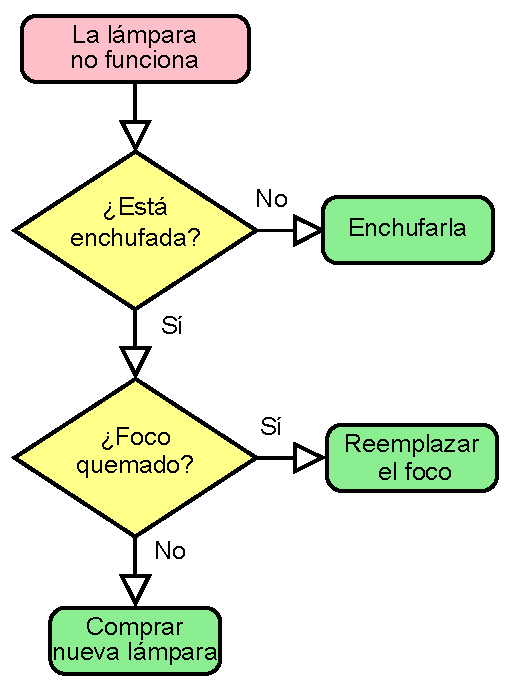
\includegraphics[scale=0.5]{pr1.pdf}
  \caption{Diagrama de flujo}
\end{figure}

\subsubsection{Sistema Binario y Decimal}

El sistema binario es un sistema de numeración que utiliza 2 símbolos 0 (cero) y 1 (uno), denominados dígitos binarios. El sistema binario, conocido también como el sistema digital, es usado para la representación de textos, datos y programas ejecutables en dispositivos informáticos.

En informática, el sistema binario es un lenguaje que utiliza 2 dígitos binarios, el 0 y el 1, donde cada símbolo constituye un bit, denominado en inglés como binary bit o bit binario. 8 bits constituyen un byte y cada byte contiene un caracter, letra o número.

Los sistemas binarios son sistemas numéricos utilizados en el área de la informática. El sistema numérico que utilizamos habitualmente es de numeración decimal, esto quiere decir, que consiste de 10 números, contando del 0 al número 9. Además,a diferencia del sistema binario, la posición que ocupa un número le otorga diferentes valores como, por ejemplo, en el número 23, el 22 representa 20 y el 3 es solo 3.

Es importante recalcar que sistema binario es un sistema de numeración de base 2 y el sistema decimal es de base 10.

Para transformar el sistema binario a decimal en este caso del binario (base 2) a decimal (base 10), se debe multiplicar cada dígito (0 o 1) del número binario, por ejemplo, 1011 por la potencia de 2 elevado a la posición que le corresponde a cada dígito comenzando con la posición 0 contando de derecha a izquierda El resultado se obtiene sumando cada multiplicación.

Siguiendo los pasos anteriores para resolver este ejercicio los pasos para convertir el código binario 1011 a sistema decimal serían:

\begin{itemize}
    \item El 1 en la posición 3 significa: multiplicar 1 por 23 cuyo resultado es 8
    \item El 0 de la posición 2 significa multiplicar 0 por 22 cuyo resultado es 0
    \item El 1 en la posición 1 significa multiplicar 1 por 21 cuyo resultado es 2
    \item El 1 en la posición 0 significa multiplicar 1 por 20 cuyo resultado es 1
\end{itemize}

se suman los resultados 8+0+2+1=11

El código binario 1011 se traduce al sistema decimal como el número 11.

Para comprobar el resultado, se invierte el proceso para transformar el número 11 en base 10 al sistema binario a base 2. Para ello se divide el número 11 por 2 hasta que sea indivisible. Luego,los restos de cada cociente de la división formarán el código binario.


\begin{definition}[Bit de paridad]
    Es un dígito binario que indica si el número de bits con un valor de 1 en un conjunto de bits es par o impar. Los bits de paridad conforman el método de detección de errores más simple.
\end{definition}

\section{Introducción a C++}
%%%%%%%%%%%%%%%%%% AGREGAR CODIGOS

\section{Problemas de optimización}

\subsection{El problema de la mochila}

Consiste en enviar a distintas partes algo, por lo que se envía de una mochila como un camión, avión, tren, etc.
Pero ésta mochila tiene que ir a diferentes destinos. Se tiene que optimizar dicho viaje
